\documentclass{article}

\usepackage{amsmath,amssymb,amsthm,graphicx,subfigure}

\pagestyle{myheadings}

\pdfpagewidth 8.5in
\pdfpageheight 11 in

\setlength\topmargin{0in}
\setlength\textheight{8.5in}
\setlength\textwidth{6.5in}
\setlength\oddsidemargin{0in}
\setlength\evensidemargin{0in}

\newcommand{\suchthat}{\ni}
\newcommand{\onlyif}{\Longleftrighttriangle}
\newcommand{\definedby}{\triangleq}
\newcommand{\union}{\bigcup}
\newcommand{\intersect}{\bigcap}
\newcommand{\where}{\mid}
\newcommand{\inverse}{\overline}

\title{CIT 596 Homework 3}
\author{Steven Tomcavage\\stomcava@seas.upenn.edu}
\date{February 17, 2011}

\markboth{\hfill Steven Tomcavage }{\hfill Steven Tomcavage }

\begin{document}

\maketitle

\section{Exercise 1.13}

Give a DFA that recognizes the language $F$ where $F$ is the language of all
strings over $\{0, 1\}$ that do not contain a pair of $1$s which are separated
by an odd number of symbols.

\begin{figure}[h!]
	\centering
	\subfigure[The NFA $A$ accepts $\inverse{F}$] {
		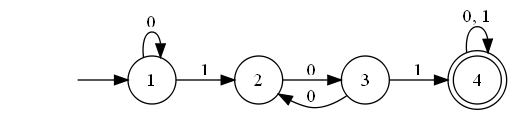
\includegraphics[height=1.0in]{1_13_a.png}
	}
	\subfigure[The DFA $B$ accepts $F$] 
	{
		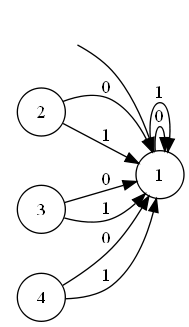
\includegraphics[height=1.0in]{1_13_b.png}
	}
	\caption{DFA for Exercise 1.13}
\end{figure}

\section{Exercise 1.16b}

Convert the given NFA (omitted) to a DFA. 

\begin{figure}[h!]
	\centering
	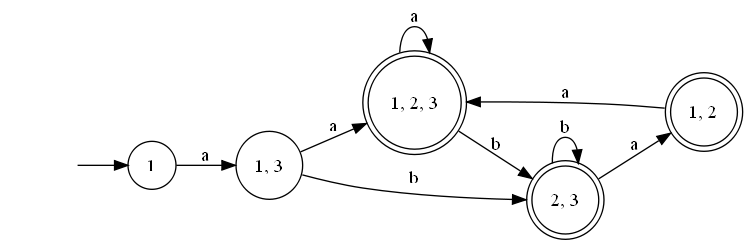
\includegraphics[height=2.0in]{1_16.png}
	\caption{DFA for Exercise 1.16b}
\end{figure}

\section{Exercise 1.17a}

Give an NFA recognizing the language $(01 \union 001 \union 010)^\star$.

\begin{figure}[h!]
	\centering
	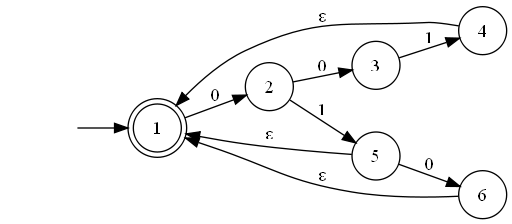
\includegraphics[height=2.0in]{1_17_a.png}
	\caption{DFA for Exercise 1.17a}
\end{figure}

\section{Exercise 1.17b}

Convert the NFA from Exercise 1.17a to an equivalent DFA.

\begin{figure}[h!]
	\centering
	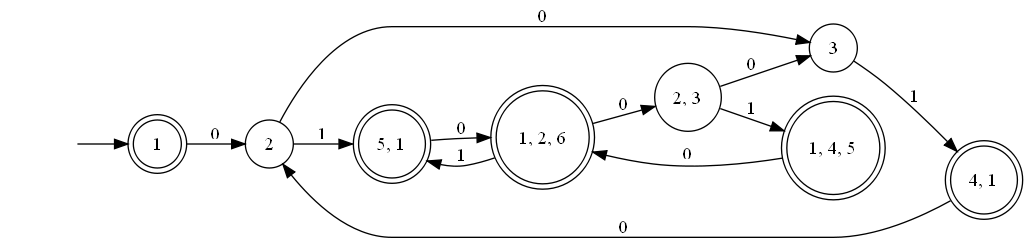
\includegraphics[height=1.5in]{1_17_b.png}
	\caption{DFA for Exercise 1.17b}
\end{figure}

\section{Exercise 1.19b}

Convert the following regular expression to an NFA: $(((00)^\star (11)) \union
01)^\star$.

\begin{figure}[h!]
	\centering
	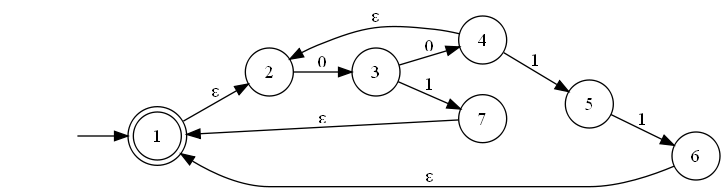
\includegraphics[height=1.5in]{1_19.png}
	\caption{DFA for Exercise 1.19b}
\end{figure}

\section{Exercise 1.21b}

Convert the following NFA to a regular expression.

\begin{figure}[h!]
	\centering
	\subfigure[The original NFA.] {
		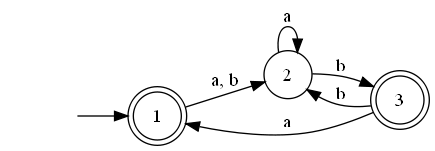
\includegraphics[height=1.5in]{1_21_a.png}
	}
	\caption{DFA for Exercise 1.21b}
\end{figure}

TODO

\section{Exercise 1.28c}

Convert the regular expression $(a \union b^+) a^+ b^+$ to an NFA, given that
$\Sigma = \{a, b\}$.

\begin{figure}[h!]
	\centering
	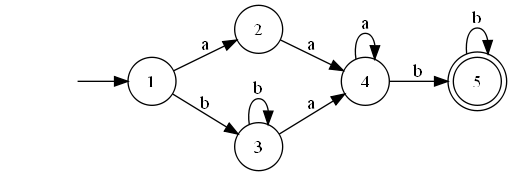
\includegraphics[height=1.5in]{1_28.png}
	\caption{DFA for Exercise 1.28c}
\end{figure}

\section{Exercie 1.29b}

Use the pumping lemma to show that the language $A_2 = \{ \omega \omega \omega
\where \omega \in \{a, b\}^\star \}$ is not regular.

Assume that $A_2$ is regular. Let $p$ be the pumping length of $A_2$. Let
$\omega = ab^pa$. So the string $ab^paab^paab^pa$ is in the language $A_2$.
Pumping $b^p$ gives $ab^pb^paab^paab^pa$, which is not in the language. Thus,
$A_2$ is not regular.

\section{Exercie 1.32}

Show that the language $B$ (omitted) is regular.

Let $w_1$ be the top row, $w_2$ be the second row, and $w_3$ be the bottom row.
Assume that the language is regular, which means that it can be pumped. Let
$p$ be the pumping length. Let $w = xy^pz$. If $B$ is regular, then $xy^py^pz$
is also in $B$.

Repeating binary sums requires examination of three cases: $0 + 0 = 0$, $0 + 1
= 1$, and $1 + 1 = 0$. Neither $0 + 0 = 0$ nor $0 + 1 = 1$ create carry-overs,
so repeating them does not affect any position to the left of those sums.
However, repeating $1 + 1 = 0$ does cause a carry-over that needs to be
considered.

TODO

\section{Exercise 1.51}

TODO

\section{Exercise 1.53}

Let $\Sigma = \{0, 1, +, =\}$ and $ADD = \{ x=y+z \where x, y, z \text{ are
binary integers and } x { is the sum of } y { and } z\}$. Show that the language
$ADD$ is not regular.

Assume that $ADD$ is regular, which means it can be pumped. Let $p$ be the
pumping length of $ADD$. Let $x=y^p + z$ be in the language $ADD$. Pumping $y$
gives $x = y^p y^p + z$ which no longer satisfies the condition that $y$ and $z$
sum to $x$. Therefore, $ADD$ cannot be pumped and is not regular.

\section{Exercise 1.55c}

What is the minimum pumping length for $001 \union 0^\star1^\star$?

The minimum pumping length is 2 because at that length, either a 0 or a 1
in the second position could be pumped. 

\section{Exercise 1.55h}

What is the minimum pumping length for $10(11^\star0)^\star0$?

The minimum pumping length is 5, where the string 10100 can be divided as $x
= 10, y = 1, z = 00$.

\end{document}
